\chapter{Modeling Paradigm}\label{ch:paradigm}

The modeling paradigm with which this repository model and simulation 
platform are implemented are described here. Implications of the 
simulation platform architecture on the design of the repository model 
are discussed and the interfaces defining components of the repository 
model follow. 

% Modeling Paradigm of Cyclus
\section{\Cyclus Simulator Paradigm }

The \Cyclus project at the \gls{UW} at Madison is the 
simulation framework in which this repository model is designed to 
operate.  Modular features within this software architecture provide a 
great deal of flexibility, both in terms of modifying the underlying 
modeling algorithms and exchanging components of a fuel cycle system.

The \Cyclus fuel cycle simulator is the  result of lessons learned 
from experience with previous nuclear fuel cycle simulation platforms.  
The modeling paradigm follows the transaction of discrete quanta of 
material among discrete facilities, arranged in a geographic and 
institutional framework, and trading in
flexible markets. Key concepts in the design of \Cyclus include open
access to the simulation engine, modularity with regard to
functionality, and relevance to both scientific and policy
analyses. The combination of modular encapsulation within the
software architecture and dynamic module loading allows for robust but 
flexible reconfiguration of the basic building blocks of a simulation 
without alteration of the simulation framework.  

The modeling paradigm adopted by \Cyclus includes a number of
fundamental concepts that comprise the bedrock on which other, more
flexible, design choices have been made. 

%%%%%%%%%%%%%%%%%%%%%%%%%%%%%%%%%%%%%%%%%%%%%%%%%%%%%%%%%%%%%%%%%%%%%%%%%%%%%%%%
\subsection{Dynamic Module Loading}

The ability to dynamically load independently constructed modules is a
heavy focus of \Cyclus development. Dynamically-loadable modules are
the primary mechanism for extending \Cyclus' capability. The primary
benefit of this approach is encapsulation: the trunk of the code is
completely independent of the individual models. Thus, any
customization or extension is implemented only in the loadable
module. A secondary benefit of this encapsulation is the ability for
contributors to choose different distribution and licensing strategies
for their contributions. By allowing models to have varied
availability, the security concerns of developers can be
assuaged (See Figure \ref{fig:repo}). 

\begin{figure}[hp!]
  \begin{center}
    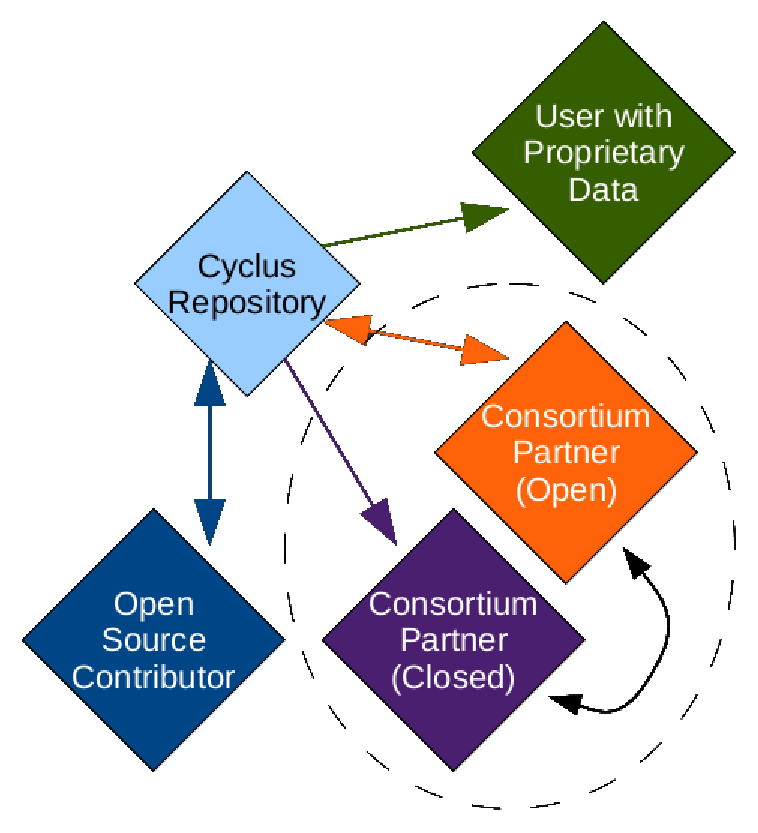
\includegraphics[height=9cm]{./chapters/paradigm/openness.eps}
  \end{center}
  \caption{The \Cyclus code repository allows for varied accessibility.}
  \label{fig:repo}
\end{figure}

Finally, this strategy allows individual developers to
explore different levels of complexity within their modules, including
wrapping other simulation tools as loadable modules within the \Cyclus 
framework. This last benefit of dynamically-loadable modules addresses 
another goal of \Cyclus: ubiquity amongst its potential user base. By
engineering \Cyclus to easily handle varying levels of complexity, a single
simulation engine can be used by both users keen on big-picture policy
questions as well as users interested in more detailed, technical
analyses.

%%%%%%%%%%%%%%%%%%%%%%%%%%%%%%%%%%%%%%%%%%%%%%%%%%%%%%%%%%%%%%%%%%%%%%%%%%%%%%%%
\subsubsection{Encapsulation}

\Cyclus implements an encapsulated structure that takes advantage of 
object-oriented software design techniques in order to create an 
extensible and modular user and developer interface. A primary 
workhorse for this implementation is the notion of dynamic module 
loading in combination with  well defined module interfaces within 
a region, institution, and facility  hierarchy. In this paradigm, 
the shared interface of polymorphic objects is abstracted from the 
logic of their instantiation by the model definition they inherit.  

In this way, \Cyclus allows a level of abstraction to exist between 
the simulation and model instantiation as well as between model 
instantiation and behavior.  An interface defines the set of shared 
functions of a set of subclasses in an abstract superclass. In \Cyclus
main superclasses are Regions, Institutions, Facilities, and Markets 
while their subclasses are the concrete available model types (e.g. a 
RecipeReactorFacility). See Figure \ref{fig:modularity}.

The interface for the FacilityModel class is the set of 
virtual functions declared in the Facility class such as getName, 
getID, executeOrder(), sendMaterial(), receiveMaterial() etc.  Through 
such an interface, the members of a subclass can be treated as 
interchangeable (polymorphic) instantiations of their shared 
superclass. 

\begin{figure}[htbp!]
  \begin{center}
    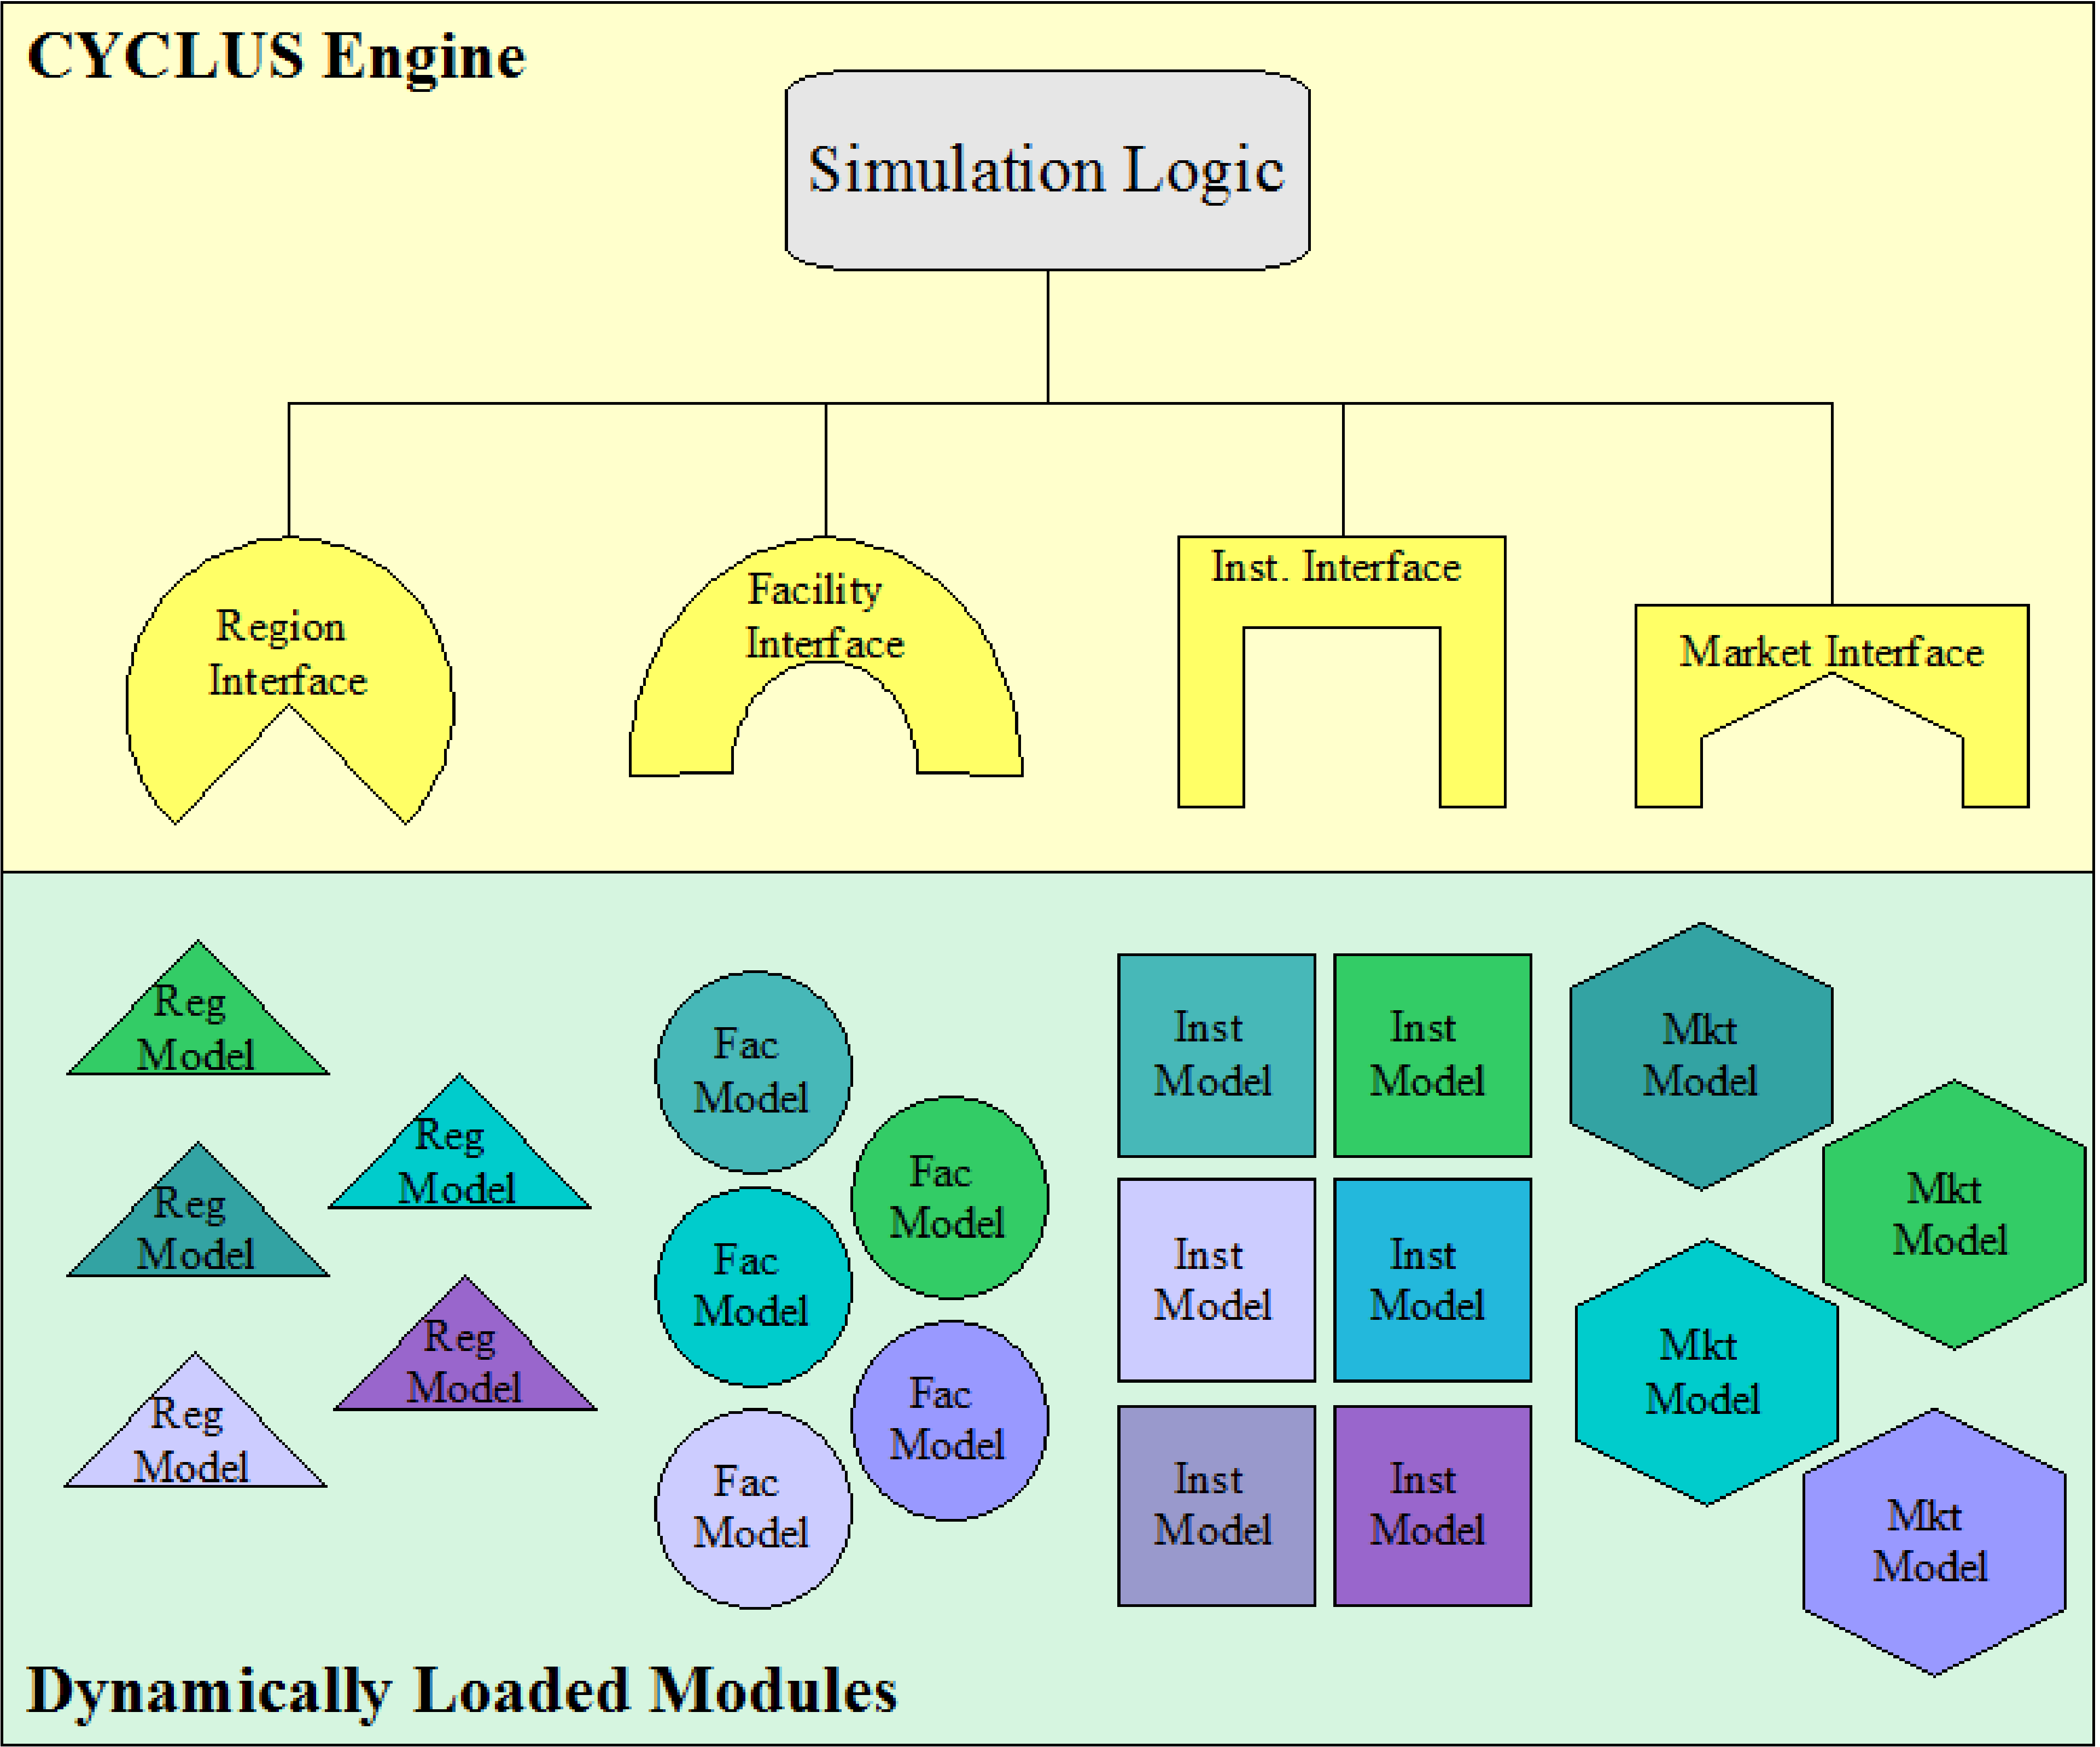
\includegraphics[height=10cm]{./chapters/paradigm/modularity.png}
  \end{center}
  \caption[Module Interfaces and Encapsulation]{Modules are defined solely 
  by their interfaces in a modular paradigm and can be arbitrarily 
  interchanged with modules posessing equivalent interfaces.}
  \label{fig:modularity}
\end{figure}


%%%%%%%%%%%%%%%%%%%%%%%%%%%%%%%%%%%%%%%%%%%%%%%%%%%%%%%%%%%%%%%%%%%%%%%%%%%%%%%%
\subsubsection{Modularity and Extensibility}

A modular code must have the traits of encapsulation and abstraction 
appropriate for a user or developer to flexibly make alterations to 
the simulation performance with minimal modification to the code. An 
extensible code should be both robustly suited to the addition of 
classes and subclasses as well as suited to communication with other codes.
In \Cyclus, addition of new models by dynamic loading is possible without 
any alteration of the software trunk. The modular design of \Cyclus stresses
avoidance of rigidity, in which changes to the code are potentially difficult, 
and fragility, in which changes to the code are potentially damaging.

%%%%%%%%%%%%%%%%%%%%%%%%%%%%%%%%%%%%%%%%%%%%%%%%%%%%%%%%%%%%%%%%%%%%%%%%%%%%%%%%
\subsection{Market-based Material Transactions}

The foundation of a simulation is a commodity market that collects 
offers and requests and matches them according to some algorithm.  The 
user is able to select which type of algorithm is used for each market 
by selecting a MarketModel and configure it with a particular set of 
parameters defined by that MarketModel.  Changing the parameters of a 
market changes its performance and selecting a different MarketModel 
completely changes its behavior.

The transaction of nuclear materials takes place in markets that act
as brokers matching a set of requests for material with a set of
offers for that material. A variety of market models will be available
to perform this brokerage role. It is important to note that each
market is defined for a single commodity and acts independently of
other markets. Once the requests and offers have been matched by each
market in a simulation, the facilities exchange material objects.

Facilities are deployed to issue offers and requests in these markets.  
Like markets, the user may select which type of algorithm is used for 
each facility by selecting a FacilityModel and configure it with a 
particular set of parameters defined by that FacilityModel.  Changing 
the parameters of a facility changes its performance and selecting a 
different FacilityModel completely changes its behavior.  Unlike 
markets, multiple independent instances of each facility configuration 
can be deployed to represent individual facilities.


%%%%%%%%%%%%%%%%%%%%%%%%%%%%%%%%%%%%%%%%%%%%%%%%%%%%%%%%%%%%%%%%%%%%%%%%%%%%%%%%
\subsection{Discrete Materials and Facilities}

The \Cyclus modeling infrastructure is designed such that every
facility in a global nuclear fuel cycle is treated and acts
individually. While modeling options exist to allow collective
action, this will be as a special case of the individual facility
basis. Each facility has two fundamental tasks: the transaction of
goods or products with other facilities and the transformation of
those goods or products from an input form to an output form.  For
example, a reactor will receive fresh fuel assemblies from a fuel
fabrication facility, transform them to used used fuel assemblies
using some approximation of the reactor physics, and supply those used
fuel assemblies to a storage facility.


A facility configuration is created by selecting a FacilityModel and 
defining the parameters for that facility configuration.
Each FacilityModel will define its own set of parameters that 

The repository model that is the subject of this work is a facility 
model within the \Cyclus simulation paradigm. 
govern its performance.  The same FacilityModel may be used for 
multiple facility configurations in the same region, each with 
parameters values appropriate for that facility configuration.

%%%%%%%%%%%%%%%%%%%%%%%%%%%%%%%%%%%%%%%%%%%%%%%%%%%%%%%%%%%%%%%%%%%%%%%%%%%%%%%%
\subsection{Materials}

Material movement is the primary unit of information in \Cyclus.  
Materials passed, traded, and modified between and within facilities 
in the simulation are recorded at every timestep.  This material 
history is stored in the output dataset of \Cyclus. In addition to 
holding the map of isotopes and their masses, a material object holds 
a comprehensive history of its own path as it moves through models 
within the simulation. 

\subsection{Implications for Repository Model}

The above sections outline the fuel cycle simulation platform
currently under development at \gls{UW} in which the repository model
at hand is to be implemented.  Implemented as a facility within this 
framework, the repository model interface is defined by the Facility
Model interface defined within the \Cyclus paradigm. 

That interface requires that a capacity be defined by the repository at every 
\Cyclus timestep so that the repository may make appropriate requests of 
disposable material.

Furthermore, the capability for dynamic module loading possible within 
the \Cyclus paradigm allows the repository system subcomponents to be 
interchangeably loaded at runtime, enabling comparison of various 
repository subcomponents, physical models of varying levels of detail. 

The repository is both a subclass and a superclass. It is a subclass of the 
FacilityModel class, and a superclass of its own subcomponents. That is, 
dynamically loaded subcomponents of the repository inherit data, parameters and 
behaviors from the repository itself. 


%%%%%%% As Paul Dirac once said. . . In science one tries to tell
%%%%%%% people, in such a way as to be understood by everyone,
%%%%%%% something that no one ever knew before. But in the case of
%%%%%%% poetry, it's the exact opposite!




\section{Repository Modeling Paradigm}

The repository model architecture is intended to modularly permit 
exchange of disposal system subcomponents, accept arbitrary spent fuel 
streams, and enable extending modules representing new or different 
component models.

\subsection{Simulation Interface}

The interface of the repository model with the \Cyclus fuel cycle 
simulation interface is intended to be minimally restrictive, 
requiring only that the simulation supply waste stream information and 
provide a bookkeeping framework with which to record repository 
performance metrics. The repository model, in order to participate in the 
simulation as a facility model, must make requests for spent material up 
to its capacity. Determination of the repository capacity for various 
types of spent fuel commodities will comprise the interfacing functionality of 
the repository model. With the intention of developing the repository model in 
such a way as to be capable of interfacing with other simulation tools, however, 
calculation of metrics including expected dose rates and 
component failures will be the model's primary functionality. 

\subsubsection{Waste Stream Input}

The repository model must accept arbitrary spent fuel and high level waste
streams.  Material objects resulting from the simulated fuel cycle arrive at 
the  repository and are emplaced if all repository capacity limits allow 
it.

Since disposable material in most simulations of interest will be of variable 
composition and therefore heterogeneous heat production capability, the 
repository model will repeatedly need to recalculate its own capacity as 
new materials are offered.

\subsubsection{Repository Performance Metrics Calculated}

Repository performance metrics that may be calculated from the source 
term and heat data calculated by the model will cover many metrics of
interest to sustainability goals. Some metrics support analyses that
seek to maximize safe repository capacity under heat and source term limitations. 
Those include spatial dimensions, spatial dimensions per kWh or equivalent,
repository footprint, and number of waste packages generated.

Still other metrics that may be calculated include those being considered by 
the \gls{UFD} campaign in a Fuel Cycle Data Package task underway 
\cite{nutt_personal_2011}. Additional metrics that will be considered in this
context will likely include environmental metrics such as peak dose 
to the public, radiotoxic fluxes released to the biosphere integrated over time, 
and the minimum managed lifetime.  These metrics are recorded in a database 
flexibly defined by the repository model. 

\subsubsection{Facility Functionality}

The repository will behave as a facility within the \Cyclus simulation 
paradigm. The fundamental facility behavior within \Cyclus involves 
participating in commodity markets. The repository will participate as 
a requester of waste commodities. During reactor operation, the 
repository will make requests to markets dealing in spent fuel streams 
according to its available capacity. Possible optional intermediate storage facility 
model is available for cooling periods.

\subsection{Nested Component Concept}

The fundamental unit of information in the repository model is the 
nuclide release at each stage of containment, and the repository model 
in this work mimics reality treating them as nested elements in a 
release chain.

\subsubsection{Control Volumes}

Each component of the repository system (i.e. waste form, waste package, buffer, 
and geologic medium) is modeled as a discrete control volume. Each control 
volume performs its own mass balance at each time step and assesses its own 
internal  heat transfer and degradation phenomena separately from the other 
nested components.

Each control volume will initially be modeled as a mixed cell. That is, for 
permeable porous media, all contaminants released into the pore and fracture 
water are assumed to be uniformly distributed.  

\subsubsection{Information Passing Between Volumes}

Each component passes some information radially outward to the nested 
component immediately containing it and some information radially 
inward to the nested component it contains.

Most component models require external information concerning the 
water volume that has breached containment, so information concerning 
incoming water volumes is passed radially inward. 

Each component model similarly requires information about the radionuclides 
released from the component it immediately contains.  Thus, nuclide 
release information is passed radially outward from the waste stream 
sequentially through each containment layer to the geosphere.

\subsubsection{Concept Generality}

The capability to allow each model to define the models within it gives this 
repository model concept the ability to model many types of repository concept 
while maintaining a simple interface with the simulation. 

\subsection{Components of the Nested System}

\subsubsection{Waste Stream}

The waste stream data object contains spent fuel isotopics over the 
course of the simulation. As radionuclides are gained, lost, and transmuted within 
the spent fuel object, a history of its isotopic composition is recorded.

For waste streams that vary from each other in composition, the thermal capacity 
of the repository must be recalculated. One way to model this will be to 
recalculate the appropriate lengthwise spacing of waste packages when the heat 
generation rate of a new package is significantly different than other waste 
packages in the repository. 

\subsubsection{Waste Form}
The waste form model will calculate nuclide release due to dissolution 
of the waste form. Various heuristics by which nuclide release is modeled in 
accordance with waste form dissolution as well as the method by which 
the dissolution is modeled.

Dissolution can be instantaneous, rate based, water dependent, heat 
dependent, or coupled.

Dissolution related release can be modeled as congruent, solubility 
limited, or both. Some radionuclides are immediately accessible, and some 
tend to remain in the fuel matrix. 

\subsubsection{Waste Package}
The waste package model calculates nuclide release due to waste 
package failure. Waste package failure is typically modeled as 
instantaneous and complete or partial and constant. That is, a delay 
before full release, or a constantly present hole in the package.

Waste package time to failure is dependent on water contact and heat, 
but can be modeled as an average, probabilistic, or a rate.

In the case of highly deforming geologic media, such as salt, 
mechanical failure can be the primary mechanism for release from the 
waste package.

\subsubsection{Buffer}
Diffusion is the primary mechanism for nuclide transport through the 
buffer component of the repository system.  

Salt, clay, and borehole repository concepts may not have a buffer 
material.

\subsubsection{Backfill}
Similarly, diffusion is the primary mechanism for nuclide transport 
through the buffer component of the repository system.

Clay concepts and borehole concepts may not have a backfill material. 


\subsubsection{Geological Environment}

The literature review introduced various hydrological models that represent
fluid and contaminant travel through permeable porous media and fractured porous 
media. These assume saturated flow and incorporate diffusive flow, advective 
flow, hydrodynamic dispersion, and equilibrium sorption. The geological 
environment control volume component will implement these models appropriately 
for each geology to provide a mass balance and to communicate concentrations to  
adjacent components.  Dirichlet boundary conditions at the surfaces of the 
control volume will allow the simulation to step through transport in the rock. 
Additional boundary condition types maybe implemented as extensions to the base 
case model.




% Modeling Paradigm of the Repository model

% Structure
% Conentric objects 
% 
% Modularity
%% Encapsulation
%% Interfaces


% The modeling paradigm is modular
%% components are within each other like a russian doll
%% Components include 
%% the waste itself,
%% the waste form,
%% the waste package,
%% the buffer,
%% the backfill, 
%% the tunnel lining,
%% the near field geology
%% and the far field geology
% Each component is defined by its interface
%% The interface is defined by the functions available to other models
%% The models within are interchangeable if they share an interface
% the interfaces between the models are based on information in and 
% out
% The
